

\section{Inference in Bayesian Networks}

Inference involves using known knowledge (evidence) to deduce new knowledge (unknown or hidden variables).

\subsection*{Steps to Construct a Bayesian Network}

\begin{enumerate}
    \item \textbf{What is observed?} (Evidence)
    \item \textbf{What do you want to find out?} (Query)
    \item \textbf{What other variables simplify the model?} (Hidden or latent variables)
\end{enumerate}

\subsection*{Hidden Variables}
Hidden variables are unobserved variables that affect the probabilities of observed or queried variables.

\subsection*{Example:}
\[
\alpha \cdot P(\text{Appointment}, \text{Light}, \text{No})
\]
Here, \( \alpha \) is a normalization constant that ensures the resulting distribution sums to 1.

\section{Marginalisation and Normalisation}

\begin{itemize}
    \item \textbf{Marginalisation:}
    \[
    P(a) = P(a, b) + P(a, \neg b)
    \]
    \item \textbf{Conditional Inference:}
    \[
    P(X \mid e) = \alpha \cdot P(X, e) = \alpha \cdot \sum_y P(X, e, y)
    \]
    where \( y \) ranges over hidden variables.
    \item \( \alpha \) is the normalisation constant.
\end{itemize}

\subsection*{Challenges}
- Inference by enumeration scales poorly with many variables.
- The complexity of exact inference depends heavily on the network’s structure.

\section{Exact and Approximate Inference Methods}

\subsection*{Exact Inference Methods}
\begin{itemize}
    \item \textbf{Inference by Enumeration}
    \item \textbf{Variable Elimination}
\end{itemize}

\subsection*{Approximate Inference Methods}
\begin{itemize}
    \item \textbf{Stochastic Simulation}
    \item \textbf{Variational Methods}
    \item \textbf{Sampling Techniques}
\end{itemize}

\section{Sampling Techniques}

Sampling is used to approximate distributions by drawing random values from them.

\subsection*{Cumulative Probability Distribution}

\begin{itemize}
    \item Example: Weather distribution
\end{itemize}

\[
\begin{aligned}
P(X = v_1) &= 0.3 \quad \text{(Sunny)} \\
P(X = v_2) &= 0.4 \quad \text{(Rainy)} \\
P(X = v_3) &= 0.1 \quad \text{(Cloudy)} \\
P(X = v_4) &= 0.2 \quad \text{(Foggy)} \\
\end{aligned}
\]

Steps:
\begin{enumerate}
    \item Order the values of the domain \( X \)
    \item Generate the cumulative distribution
    \item Draw a random number \( y \sim \text{Uniform}(0,1) \)
    \item Select the value of \( X \) based on where \( y \) falls in the cumulative distribution
\end{enumerate}

\subsection*{Rejection Sampling}
\begin{itemize}
    \item Generate full samples.
    \item Reject samples that do not match the evidence.
    \item Inefficient if evidence is rare.
\end{itemize}

\subsection*{Likelihood Weighting}
\begin{itemize}
    \item Fix the evidence variables.
    \item Sample other variables conditioned on evidence.
    \item Weight each sample by its likelihood.
\end{itemize}

\subsection*{Importance Sampling}
\begin{itemize}
    \item Draw samples from an easier distribution.
    \item Weight the samples to correct the bias.
\end{itemize}

\section{Uncertainty Over Time: Markov Models}

\subsection*{Markov Assumption}
The current state depends only on a finite number of previous states.

\subsection*{Markov Chain}
A sequence of random variables \( X_1, X_2, \dots, X_n \) satisfying:

\[
P(X_{t+1} \mid X_t, X_{t-1}, \dots, X_1) = P(X_{t+1} \mid X_t)
\]

\textbf{Key Assumption:} The future is independent of the past given the present.

\subsection*{Transition Model}
\[
P(X_{t+1} \mid X_t)
\]

\begin{center}
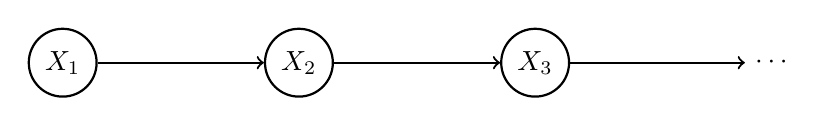
\begin{tikzpicture}[->, thick, node distance=3cm]
  \node[draw, circle] (x1) {$X_1$};
  \node[draw, circle, right of=x1] (x2) {$X_2$};
  \node[draw, circle, right of=x2] (x3) {$X_3$};
  \node[draw=none, right of=x3] (dots) {$\cdots$};

  \draw (x1) -- (x2);
  \draw (x2) -- (x3);
  \draw (x3) -- (dots);
\end{tikzpicture}
\end{center}


\section{Hidden Markov Models (HMMs)}

\subsection*{Definition}
A Markov model with hidden (unobservable) states.

\begin{itemize}
    \item \textbf{Transition Probability:} \( P(X_{t+1} \mid X_t) \)
    \item \textbf{Emission (Sensor) Probability:} \( P(E_t \mid X_t) \)
\end{itemize}

\subsection*{Sensor Markov Assumption}
Current observation depends only on the current state.

\subsection*{Tasks in HMMs}
\begin{itemize}
    \item \textbf{Filtering:} Estimate current state given past observations
    \item \textbf{Prediction:} Estimate future states
    \item \textbf{Smoothing:} Estimate past states
    \item \textbf{Most Likely Explanation:} Find the most likely sequence of hidden states
\end{itemize}

\begin{center}
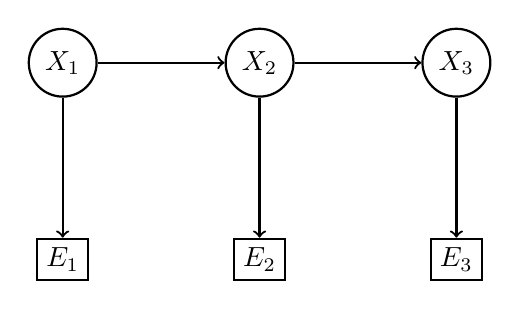
\begin{tikzpicture}[->, thick, node distance=2.5cm]
  % Hidden states
  \node[draw, circle] (h1) {$X_1$};
  \node[draw, circle, right of=h1] (h2) {$X_2$};
  \node[draw, circle, right of=h2] (h3) {$X_3$};

  % Observed states
  \node[draw, rectangle, below of=h1] (e1) {$E_1$};
  \node[draw, rectangle, below of=h2] (e2) {$E_2$};
  \node[draw, rectangle, below of=h3] (e3) {$E_3$};

  % Arrows between hidden states
  \draw (h1) -- (h2);
  \draw (h2) -- (h3);

  % Arrows from hidden to observed
  \draw (h1) -- (e1);
  \draw (h2) -- (e2);
  \draw (h3) -- (e3);
\end{tikzpicture}
\end{center}


\section{Language Models}

\subsection*{Simple Models: Bag of Words and Unigrams}

\begin{itemize}
    \item Words are treated as independent.
    \item \( P(w_i) \): Probability distribution over words.
    \item Frequency vector indicates word usage.
\end{itemize}

\subsection*{Bigram Models}

\[
P(w_i \mid w_{i-1})
\]

\begin{itemize}
    \item The domain of each variable is the vocabulary.
    \item Models word sequences using adjacent word pairs.
\end{itemize}

\subsection*{Trigram Models}

\[
P(w_i \mid w_{i-1}, w_{i-2})
\]

\subsection*{N-gram Models}

\begin{itemize}
    \item Extend bigrams/trigrams to any \( n \)-length sequence.
    \item Capture local dependencies in language.
\end{itemize}

\subsection*{Limitations of N-gram Models}

\begin{itemize}
    \item \textbf{Sparsity:} Many possible sequences are never seen in training data.
    \item \textbf{Data Size:} Large corpora are needed to get reliable estimates.
    \item \textbf{Lack of Semantic Understanding:} Words are treated as symbols, ignoring meaning and context.
    \item \textbf{Lack of Global Information:} Limited context prevents understanding long-distance dependencies.
\end{itemize}
